\documentclass[12pt]{article} 

\usepackage{tikz}

\begin{document}

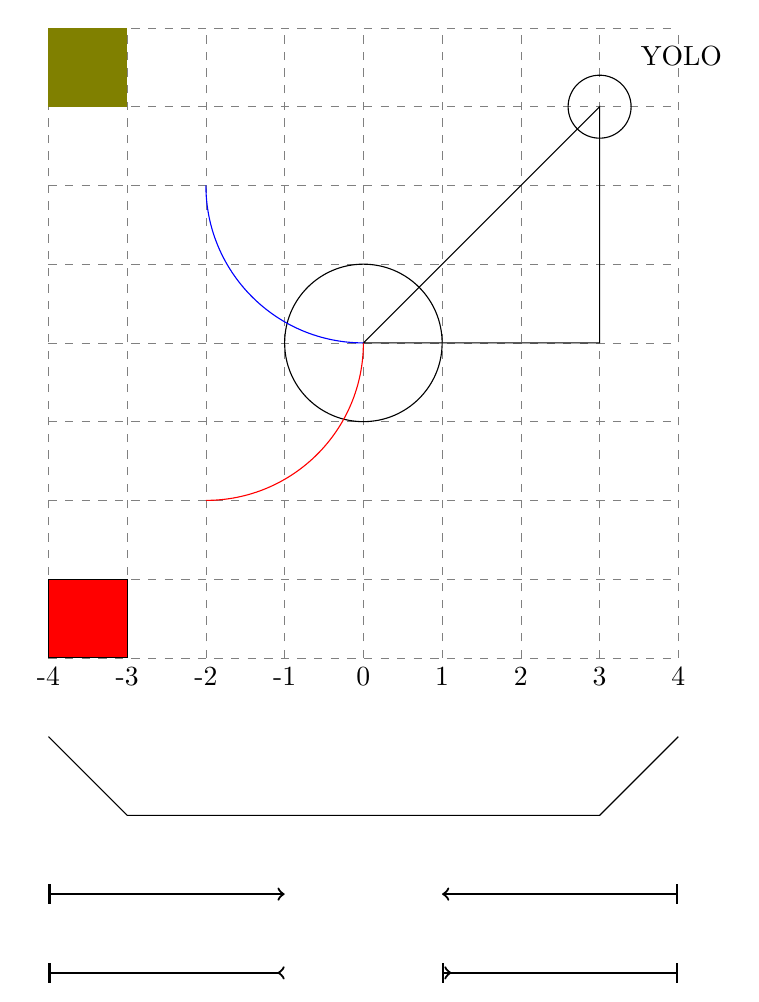
\begin{tikzpicture}
  % Make a grid
  \draw[step=1,gray,very thin, dashed] (-4,-4) grid (4,4);
  % Make a rectangle (`cycle` makes a line between the first and last points)
  \draw (0,0) -- (3,3) -- (3,0) -- cycle;
  % Make a circle at origin with radius 1
  \draw (0,0) circle (1);
  \draw (3,3) circle (0.4);
  % Make an arc with the starting point at origin 
  \draw[red] (0,0) arc (0:-90:2); % from 0 to -90 degrees, with radius=2
  \draw[blue] (0,0) arc (-90:-180:2);
  % Fill a rectangle with 50% red and 50% green
  \fill[red!50!green] (-4,4) rectangle (-3,3);
  % Fill and draw at the same time 
  \filldraw[fill=red, draw=black] (-4,-4) rectangle (-3,-3);
  % Make a line
  \draw (-4,-5) -- (-3,-6) -- (-3,-6) -- (3,-6) -- (4,-5) ;
  % A few arrow styles
  \draw[thick,|->] (-4,-7) -- (-1,-7) ;
  \draw[thick,<-|] (1,-7) -- (4,-7) ;
  \draw[thick,|-<] (-4,-8) -- (-1,-8) ;
  \draw[thick,|>-|] (1,-8) -- (4,-8) ;
  % Add an annotation
  \draw (3.4,3.4) node[anchor=south west] {YOLO} ;
  % Write grid numbers
  \foreach \x in {-4,-3,-2,-1,0,1,2,3,4}
    \draw (\x,-4) node[anchor=north] {\x} ;
\end{tikzpicture}

\end{document}
